
    \begin{abstract_online}{Effect of Alkyl chain on The Wetting Behavior of Aqueous Ionic Liquids: A Molecular Dynamics Study }{%
        \underline{S. Bhattacharjee}, D. Chakraborty, S. Khan}{%
        }{%
        Department of Chemical & Biochemical Engineering, IIT Patna, India}
    We report a Molecular Dynamics investigation on the effect of alkyl chain on wetting and interfacial properties of aqueous imidazolium-based ionic liquids (ILs), consisting 1-ethyl-3- methylimidazolium [EMIM], 1-butyl-3-methylimidazolium, [BMIM] and 1-Hexyl-3-methylimidazolium [HMIM] cations with common tetra fluoroborate anion. Effect of alkyl chain length on wetting behavior of aqueous IL within concentration range of $10–30 \ wt \%$ IL were studied (Figure 1). The difference between the contact angle for aqueous $[EMIM][BF_4]$ and $[BMIM][BF_4]$ droplets are small, irrespective of $wt \%$ of IL. However, drastic decrease in the contact angle was observed for long alkyl chain $[HMIM][BF_4]$. Droplet characteristics near the surface were investigated by profiling the density perpendicular (z-direction) and horizontal (r-direction) to the graphite sheet; which was further quantified by an orientation order parameter. Most of IL molecules are found near the graphite surface for all the cases. However, presence of longer alkyl $[HMIM][BF_4]$ and $[BMIM][BF_4]$ are found in the liquid-vapor interface, which are in agreement with the literature1–3 which deals with aqueous solutions of IL at solution/vapor interface . Further, hydrogen bond analysis between IL and water at different $wt \%$ are also investigated. Chain length of cation, and interfacial tensions of aqueous ILs which has been compared with the experimental values [4,5] are the crucial factors for wetting behavior of aqueous IL in our study. In addition to that, we have also investigate the electrowetting behavior of ionic liquid droplet at different strengths of electric field. \begin{center}  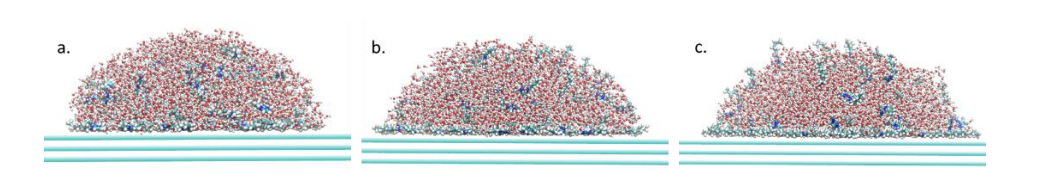
\includegraphics[width=\linewidth]{abstracts/txt/figures/sanchari.png}  \caption{\textbf{Figure 1:} Snapshot of $30 \ wt \%$ of aqueous a) $[EMIM][BF_4]$ b) $[BMIM][BF_4]$ c) $[HMIM][BF_4]$}  \end{center}  
    
        \textbf{References} \newline{}[1]Chaumont A, et al., The Journal of Physical Chemistry B , 109 (40)(2005), 18964–18973. \newline{}[2]Chevrot G, et al., Physical Chemistry Chemical Physics, 8 (36)(2006), 4166–4174. \newline{}[3]Picálek J, et al., Physical Chemistry Chemical Physics, 10 (37)(2008), 5765–5775 \newline{}[4]Rilo E, et al., O. Fluid Phase Equilibria, 285 (1–2)(2009), 83–89. \newline{}[5]Shojaeian A, Thermochimica acta, 673(2019), 119–128.  
    \end{abstract_online}
    